% =================================================
% 性学系列 · BDSM 与 Kink
% 共享基座见 common.tex
% =================================================
\documentclass[12pt,UTF8,openany]{ctexbook}
% =================================================
% common.tex —— 性学系列 共享基座
% 导言区 / 配色 / TikZ 库 / ctexset / C 列型 / 字体 / 书眉页码
% 各册 % =================================================
% common.tex —— 性学系列 共享基座
% 导言区 / 配色 / TikZ 库 / ctexset / C 列型 / 字体 / 书眉页码
% 各册 % =================================================
% common.tex —— 性学系列 共享基座
% 导言区 / 配色 / TikZ 库 / ctexset / C 列型 / 字体 / 书眉页码
% 各册 \input{common.tex} 引用
% =================================================
\usepackage[top=2.5cm,bottom=2.5cm,left=2.6cm,right=2.6cm,headheight=2.0cm]{geometry}
\usepackage{amsmath}
\usepackage{amssymb}
\usepackage{array}
\usepackage{tabularx}
\usepackage{multirow}
\usepackage{booktabs}
\usepackage{enumitem}
\usepackage{xcolor}
\usepackage{graphicx}
\usepackage{tikz}
\usetikzlibrary{positioning,calc,arrows.meta,shapes.geometric,matrix}
\definecolor{myblue}{HTML}{185FA5}
\definecolor{myblueL}{HTML}{E6F1FB}
\definecolor{mygreen}{HTML}{3B6D11}
\definecolor{mygreenL}{HTML}{C0DD97}
\definecolor{myteal}{HTML}{1D9E75}
\definecolor{myamber}{HTML}{854F0B}
\definecolor{myamberL}{HTML}{FAEEDA}
\definecolor{myred}{HTML}{A32D2D}
\definecolor{myredL}{HTML}{FCEBEB}
\definecolor{mypurple}{HTML}{534AB7}
\definecolor{mypurpleL}{HTML}{EEEDFE}
\definecolor{mycoral}{HTML}{D85A30}
\definecolor{mycoralL}{HTML}{FAECE7}
\definecolor{mypink}{HTML}{D4537E}
\definecolor{mypinkL}{HTML}{F4C0D1}
\definecolor{mypinkM}{HTML}{ED93B1}
\definecolor{mygray}{HTML}{888780}

% 字体
\setCJKfamilyfont{hei}{SimHei}
\newcommand{\myhei}{\CJKfamily{hei}}

% 书眉与页码（印刷友好：中文页眉 + 居中页码）
\usepackage{fancyhdr}
\pagestyle{fancy}
\fancyhf{}
\fancyhead[L]{\small\myhei 性学系列}
\fancyhead[R]{\small\leftmark}
\fancyfoot[C]{\small\thepage}
\renewcommand{\headrulewidth}{0.4pt}
\fancypagestyle{plain}{\fancyhf{}\fancyfoot[C]{\small\thepage}\renewcommand{\headrulewidth}{0pt}}
\fancypagestyle{empty}{\fancyhf{}\renewcommand{\headrulewidth}{0pt}}

% 行距（零基础易读，略松）
\linespread{1.3}

% 超链接：印刷友好（黑色，电子版仍可点击）
\usepackage[colorlinks,linkcolor=black,citecolor=black,urlcolor=black]{hyperref}

\ctexset{
  chapter/name={第,章},
  chapter/number={\arabic{chapter}},
  section/format=\Large\bfseries,
}

\newcolumntype{C}{>{\centering\arraybackslash}X}
 引用
% =================================================
\usepackage[top=2.5cm,bottom=2.5cm,left=2.6cm,right=2.6cm,headheight=2.0cm]{geometry}
\usepackage{amsmath}
\usepackage{amssymb}
\usepackage{array}
\usepackage{tabularx}
\usepackage{multirow}
\usepackage{booktabs}
\usepackage{enumitem}
\usepackage{xcolor}
\usepackage{graphicx}
\usepackage{tikz}
\usetikzlibrary{positioning,calc,arrows.meta,shapes.geometric,matrix}
\definecolor{myblue}{HTML}{185FA5}
\definecolor{myblueL}{HTML}{E6F1FB}
\definecolor{mygreen}{HTML}{3B6D11}
\definecolor{mygreenL}{HTML}{C0DD97}
\definecolor{myteal}{HTML}{1D9E75}
\definecolor{myamber}{HTML}{854F0B}
\definecolor{myamberL}{HTML}{FAEEDA}
\definecolor{myred}{HTML}{A32D2D}
\definecolor{myredL}{HTML}{FCEBEB}
\definecolor{mypurple}{HTML}{534AB7}
\definecolor{mypurpleL}{HTML}{EEEDFE}
\definecolor{mycoral}{HTML}{D85A30}
\definecolor{mycoralL}{HTML}{FAECE7}
\definecolor{mypink}{HTML}{D4537E}
\definecolor{mypinkL}{HTML}{F4C0D1}
\definecolor{mypinkM}{HTML}{ED93B1}
\definecolor{mygray}{HTML}{888780}

% 字体
\setCJKfamilyfont{hei}{SimHei}
\newcommand{\myhei}{\CJKfamily{hei}}

% 书眉与页码（印刷友好：中文页眉 + 居中页码）
\usepackage{fancyhdr}
\pagestyle{fancy}
\fancyhf{}
\fancyhead[L]{\small\myhei 性学系列}
\fancyhead[R]{\small\leftmark}
\fancyfoot[C]{\small\thepage}
\renewcommand{\headrulewidth}{0.4pt}
\fancypagestyle{plain}{\fancyhf{}\fancyfoot[C]{\small\thepage}\renewcommand{\headrulewidth}{0pt}}
\fancypagestyle{empty}{\fancyhf{}\renewcommand{\headrulewidth}{0pt}}

% 行距（零基础易读，略松）
\linespread{1.3}

% 超链接：印刷友好（黑色，电子版仍可点击）
\usepackage[colorlinks,linkcolor=black,citecolor=black,urlcolor=black]{hyperref}

\ctexset{
  chapter/name={第,章},
  chapter/number={\arabic{chapter}},
  section/format=\Large\bfseries,
}

\newcolumntype{C}{>{\centering\arraybackslash}X}
 引用
% =================================================
\usepackage[top=2.5cm,bottom=2.5cm,left=2.6cm,right=2.6cm,headheight=2.0cm]{geometry}
\usepackage{amsmath}
\usepackage{amssymb}
\usepackage{array}
\usepackage{tabularx}
\usepackage{multirow}
\usepackage{booktabs}
\usepackage{enumitem}
\usepackage{xcolor}
\usepackage{graphicx}
\usepackage{tikz}
\usetikzlibrary{positioning,calc,arrows.meta,shapes.geometric,matrix}
\definecolor{myblue}{HTML}{185FA5}
\definecolor{myblueL}{HTML}{E6F1FB}
\definecolor{mygreen}{HTML}{3B6D11}
\definecolor{mygreenL}{HTML}{C0DD97}
\definecolor{myteal}{HTML}{1D9E75}
\definecolor{myamber}{HTML}{854F0B}
\definecolor{myamberL}{HTML}{FAEEDA}
\definecolor{myred}{HTML}{A32D2D}
\definecolor{myredL}{HTML}{FCEBEB}
\definecolor{mypurple}{HTML}{534AB7}
\definecolor{mypurpleL}{HTML}{EEEDFE}
\definecolor{mycoral}{HTML}{D85A30}
\definecolor{mycoralL}{HTML}{FAECE7}
\definecolor{mypink}{HTML}{D4537E}
\definecolor{mypinkL}{HTML}{F4C0D1}
\definecolor{mypinkM}{HTML}{ED93B1}
\definecolor{mygray}{HTML}{888780}

% 字体
\setCJKfamilyfont{hei}{SimHei}
\newcommand{\myhei}{\CJKfamily{hei}}

% 书眉与页码（印刷友好：中文页眉 + 居中页码）
\usepackage{fancyhdr}
\pagestyle{fancy}
\fancyhf{}
\fancyhead[L]{\small\myhei 性学系列}
\fancyhead[R]{\small\leftmark}
\fancyfoot[C]{\small\thepage}
\renewcommand{\headrulewidth}{0.4pt}
\fancypagestyle{plain}{\fancyhf{}\fancyfoot[C]{\small\thepage}\renewcommand{\headrulewidth}{0pt}}
\fancypagestyle{empty}{\fancyhf{}\renewcommand{\headrulewidth}{0pt}}

% 行距（零基础易读，略松）
\linespread{1.3}

% 超链接：印刷友好（黑色，电子版仍可点击）
\usepackage[colorlinks,linkcolor=black,citecolor=black,urlcolor=black]{hyperref}

\ctexset{
  chapter/name={第,章},
  chapter/number={\arabic{chapter}},
  section/format=\Large\bfseries,
}

\newcolumntype{C}{>{\centering\arraybackslash}X}


\begin{document}

% ===== 封面 =====
\begin{titlepage}
\centering
\vspace*{1.5cm}
\begin{tikzpicture}
\draw[myblue,line width=2pt] (0,0) circle (1.2);
\node[text=white] at (0,0) {\myhei\zihao{3}性};
\end{tikzpicture}
\vspace{0.6cm}
\noindent\rule{\textwidth}{0.4pt}
\vspace{0.5cm}
\myhei\zihao{5} 性学系列\,·\,家庭健康科普\,·\,全五册
\vspace{2.5cm}
\myhei\zihao{0} BDSM 与 Kink\par
\vspace{1.2cm}
\itshape\zihao{3} 安全框架下的亲密表达\par
\vspace{5.2cm}
\noindent\rule{\textwidth}{0.4pt}
\vspace{0.5cm}
\zihao{5} 性学系列\,·\,\today
\end{titlepage}

% ===== 免责声明 =====
\begin{center}\zihao{5}\itshape
本书为家庭健康科普读物，内容力求科学严谨，但\textbf{不替代专业医生的诊断与治疗}。\\
涉及个人健康问题，请以正规医疗机构的检查与建议为准。\\
全书以安全、自愿、相互尊重为底色，尊重多元与个体差异。\par\end{center}
\clearpage

% ===== 如何使用本书 =====
\chapter*{如何使用本书}
\addcontentsline{toc}{chapter}{如何使用本书}
\noindent\textbf{性学系列共五册：}
\begin{itemize}[leftmargin=2em]
\item \textbf{A 性健康基础} —— 认知、同意、防护、STI、避孕总论（建议先读）
\item \textbf{B 亲密实践与技巧} —— 前戏、体位、高潮引导、呼吸与盆底
\item \textbf{C 男性性健康} —— 男性解剖、ED/自慰、绝育、不育
\item \textbf{D 女性性健康} —— 女性解剖、妇科、不孕、人流、避孕、孕期/更年期
\item \textbf{E BDSM 与 Kink} —— 安全框架下的亲密表达
\end{itemize}
\vspace{0.6em}
\noindent\textbf{建议阅读路径（零基础）：} 先通读 A 建立认知与安全底线 → 按需读 C 或 D 了解自己的身体 → 再读 B 学技巧 → 兴趣到了再读 E。每章末有“一页要点”可快读。
\clearpage

% ===== 目录 =====
\tableofcontents
\clearpage
\chapter{BDSM 与 Kink：安全框架下的亲密表达}
\label{chap:bdsm}

\section{一、先正名：BDSM 是什么}

\textbf{BDSM} = Bondage \& Discipline（束缚与纪律）+ Dominance \& Submission（主导与臣服）+ Sadism \& Masochism（施虐与受虐），是对一类\textbf{非传统亲密实践}的总称；圈内更宽泛的用词是 \textbf{kink（癖好）}。三个关键认知先立住：

\begin{itemize}
  \item \textbf{不是"另一种性"，是亲密表达的谱系之一}。它与"普通性爱"不是替代关系，而是光谱上的不同位置。有人一辈子只玩轻 kink（眼罩、轻拍打、角色游戏），有人玩到窒息、医疗服从——都是正常范围。
  \item \textbf{DSM-5 的关键去病理化（2013 起）}：此前 APA 把"性施虐/受虐"列为 paraphilias（性偏好）；DSM-5 起把"性偏好（paraphilia）"与"\textbf{性偏好障碍（paraphilic disorder）}"区分开——\textbf{只有当偏好带来显著痛苦、或明显影响生活功能时才算障碍}。BDSM 本身不再被默认"是病"。
  \item \textbf{远比想象中普遍}：Indiana University 对 2021 名美国成年人的研究中——拍打 30\%、dom/sub 角色 22\%、束缚 20\%、鞭打 13\%；41 国 31.7 万人调查中约 20\% 用过眼罩/束缚。也就是说，"有 kink 元素"是\textbf{多数成年人的经验}，只是多数人一辈子只在私下进行、不告诉他人。
\end{itemize}

\section{二、常见形式：不是清单，是光谱}

Kink 不是一份清单，而是\textbf{光谱}。大致分三档（每档内组合差异极大，每个人不同）：

\begin{tabularx}{\textwidth}{lX}
\toprule
\textbf{强度} & \textbf{典型内容与主要风险点} \\
\midrule
Light（轻） & 角色游戏、眼罩、耳语、轻拍打、温柔束缚——主要风险是\textbf{情绪（aftercare）与隐私}。 \\
Medium（中） & 鞭打、温度（蜡烛/冰块）、体位控制、感官剥夺——注意\textbf{皮肤/软组织损伤、束缚过紧}。 \\
Deep（深） & 窒息、医疗服从、长时间束缚、多伙伴——\textbf{窒息、神经/血流、感染}，需要经验与准备。 \\
\bottomrule
\end{tabularx}

\vspace{0.5em}
\noindent\textbf{关键：} 三档之间没有绝对界限，"deep"不是"更厉害"，只是\textbf{风险类型不同}。多数人一辈子只在 light 到 medium 之间。

\section{三、安全框架：SSC 与 RACK}

BDSM 的安全不是"小心一点"，而是一套\textbf{可执行的协议}：

\begin{itemize}
  \item \textbf{SSC}：Safe（安全）、Sane（理智）、Consensual（自愿）——圈内最经典的三原则。
  \item \textbf{RACK}：Risk-Aware Consensual Kink（\textbf{知情风险}下的自愿 kink）——比 SSC 更精细，强调"双方都知道风险是什么、能承担、才做"。
\end{itemize}

无论用哪个框架，都落到\textbf{三个动作}：\textbf{事前谈判}（hard limits 绝对不做 / soft limits 视情况 / 想要什么 / 有无基础病如心血管·糖尿病·哮喘·癫痫·凝血问题）、\textbf{事中纪律}（安全词、节奏与观察、任何"不对"就停）、\textbf{事后关怀}（aftercare，见第六节）。

\section{四、五大风险与医学依据}

\subsection*{1. 窒息（最高危，单独列）}
\textbf{颈压}：颈动脉窦是颈动脉分叉处的压力感受器，受压会触发\textbf{颈动脉窦反射}——迷走神经兴奋，心率骤降、血压骤降。三型：
\begin{itemize}
  \item \textbf{心脏抑制型（迷走型）}：占 50--70\%，可致心率降至 40 次/分以下甚至短暂心脏停搏；
  \item \textbf{血管抑制型}：5--10\%，血压骤降；
  \item \textbf{中枢型（脑型）}：晕厥伴抽搐。
\end{itemize}
60 岁以上晕厥患者中 17.6\% 与颈动脉窦相关，70 岁以上达 25\%；常见触发为扼颈、勾肩、亲吻颈部、衣领过紧、颈部按摩。\textbf{口鼻阻塞}则导致脑缺氧。系统综述（2010，48 例 CiRCA 案例）显示：绝大多数颈压猝死其实\textbf{合并脑缺氧}（颈动脉血流完全阻断），纯反射单独致死罕见——但风险依然不可控。圈内共识：\textbf{新手不做颈压与窒息；若进行，必须有人全程在场}。高危人群：老年、动脉硬化、糖尿病、正在服降压/抗心律失常药、酒精影响后。

\subsection*{2. 束缚}
主要风险是\textbf{血液循环受阻}（远端发白/发紫、发凉）与\textbf{神经压迫}（腕管、尺神经、坐骨神经——出现"麻、木、针刺"立即松开）。四肢持续束缚\textbf{不建议超过 30--60 分钟}，其间观察颜色/温度/感觉。工具选择：软绳 $>$ 皮革 $>$ 金属，避免细绳勒进皮肤。

\subsection*{3. 疼痛与软组织损伤}
淤青（皮下出血）是\textbf{正常}，数周内消退。\textbf{警惕}：皮肤破损出血、大面积淤青不退、疼痛超一周——可能是深部组织损伤或凝血问题。糖尿病/凝血问题/正在用抗凝药者，深拍打需谨慎。

\subsection*{4. 情绪回落（sub drop / dom drop）}
高强度 BDSM 后，\textbf{双方}都可能经历 30 分钟到数小时的\textbf{情绪低谷}——低落、脆弱、想哭、疲惫。机制是\textbf{催产素、多巴胺、内啡肽在峰值后回落}。\textbf{不是"矫情"，是神经内分泌的正常反应}，处理见第六节 aftercare。

\subsection*{5. 传染}
任何涉及体液/共用器具的场景，感染风险与主流性行为一致；屏障工具（安全套/避孕套、dental dam）在 BDSM 里同样适用；共用器具前后清洗/换套。

\section{五、安全词：为什么需要、怎么设}

\textbf{为什么}：在高强度感官刺激、感官剥夺或主导-臣服角色下，"不"和"疼"可能\textbf{失效}——身体在"兴奋"与"疼痛"的信号会混淆，当事人可能本能地"忍着"，而对方无法分辨。安全词就是\textbf{一个事先约定的、在情境外、明确的停/降档信号}。

\textbf{怎么设}：
\begin{itemize}
  \item \textbf{红绿灯}（最常用）：\textcolor{mygreen}{绿} = 继续；\textcolor{myamber}{黄} = 慢一点/换个方向；\textcolor{myred}{红} = \textbf{立刻停}（不管进行到哪一步）。
  \item \textbf{水果词}（避免和"不"混淆）：预先约定两个词，如"菠萝 = 慢"、"芒果 = 停"——好处是"疼""不要"不会被误读。
  \item \textbf{纪律}：说了安全词，\textbf{无条件停下、检查、再谈}——这是 SSC 的底线。
\end{itemize}

\section{六、Aftercare（事后关怀）}

\textbf{是什么}：BDSM 结束后\textbf{一段刻意安排的关怀时间}，通常 30 分钟到数小时。\textbf{为什么}：OT/DA 峰值后回落，双方（dom 与 sub）都易进入情绪低谷（sub drop / dom drop），此时身体敏感、情感脆弱；aftercare 是给这段回落一个\textbf{"软着陆"}。\textbf{做什么}（按需求，不是清单）：温暖（毯子、拥抱）、补水吃点东西、轻声确认"你还好吗"、一起清理并慢慢离开场景、事后 24 小时内的正常关怀——不是"翻旧账"，而是把关系接回日常。\textbf{常见误区}：aftercare 只给 sub——\textbf{dom 也需要}，很多 dom 事后情绪回落同样明显。

\section{七、常见误区}

\begin{tabularx}{\textwidth}{lX}
\toprule
\textbf{误区} & \textbf{事实} \\
\midrule
"BDSM = 性变态" & DSM-5 起已区分"偏好"与"障碍"；只有带来显著痛苦/功能受损才算障碍。 \\
"痛苦 = 高潮" & 愉悦是\textbf{心理 + 生理 + 关系}多维的，不是单纯的痛。 \\
"只有特定性别/性取向才玩" & 所有性别和性取向都有 kink 玩家。 \\
"一定要用道具" & 眼神、耳语、节奏、呼吸都是 kink。 \\
"一定要玩很大" & 光谱上 light 完全够用，不必升级。 \\
"第一次就玩 deep" & 经验、信任、沟通是前提，deep 需要时间积累。 \\
\bottomrule
\end{tabularx}

\section{八、和主流性爱的关系}

\textbf{不是替代、不是升级、不是堕落}——是亲密表达的\textbf{一个维度}。你和伴侣可以一辈子只玩 light（角色游戏、眼罩、轻拍打），或只在特定场景玩，或完全不玩——都完全正常。\textbf{关键}：kink 是\textbf{加分项}，不是\textbf{必选项}。

\section{九、何时需要专业帮助}

当它变成\textbf{强迫性}（不做就难受、做就停不下来）；成为\textbf{唯一能唤起}的方式且明显影响关系；有\textbf{创伤史}、触发时反应剧烈并影响日常；或伴随\textbf{反复疼痛/损伤}且找不到原因——找\textbf{正规性医学科/心理科}，别把"圈内咨询师"当唯一渠道。

\section{十、红旗信号（立刻停下）}

\begin{itemize}
  \item 说了安全词，对方不停；
  \item 束缚超过 1 小时，远端发白/发紫；
  \item 颈部受压后头晕、视物模糊、心率异常；
  \item 皮肤大面积破损，或疼痛超过一周不退；
  \item 事后 24 小时情绪仍显著低落且无法自我调节。
\end{itemize}

\section{一页速查}

\begin{tabularx}{\textwidth}{lX}
\toprule
\textbf{项目} & \textbf{要点} \\
\midrule
安全框架 & SSC / RACK。 \\
事前 & hard/soft limits、基础病筛查。 \\
安全词 & 红绿灯或水果词；说了无条件停。 \\
窒息 & 新手不做颈压；若进行须有人全程在场。 \\
束缚 & 30--60 分钟上限；观察颜色/温度/感觉。 \\
Aftercare & 30 分钟到数小时；\textbf{双方都需要}。 \\
传染 & 屏障工具同样适用。 \\
就医 & 强迫性/唯一唤起/反复损伤/创伤史。 \\
\bottomrule
\end{tabularx}

\vspace{1em}
\noindent\textbf{一句话总结：} BDSM 不是"另一种性"，是亲密表达的\textbf{一个维度}——\textbf{SSC/RACK + 安全词 + aftercare} 三件套到位，它就和任何亲密行为一样，可以既愉悦又安全。

\chapter{非常性爱：非主流亲密玩法}
什么想法，非常性爱的活力正在改变着这个时代。那些曾被认为是走在狂野边缘的事情，如今却被当作平淡乏味的事。想想大街上卖的绒毛手帕，拿性玩具当谈话主题的电视节目，透明内衣设计师，还有人全身上下都打洞！
尽管你也许没有兴趣用鞭子把你的男友打成性狂暴者，或是打扮成法国女佣的模样，但只要你跟大多数人一样，那对于非常性爱以及它对性生活的影响，你的好奇心可不会只有一点而已。
显然这并不是每个人都适合做的，但是加入一点古怪的小把戏，是为你的性经历增添活力的最快方法。还好，这并不是要你到还未有人涉足的领域去探险（有人适过在潜水时戴着呼吸器隔着衣服做爱吗？），只是尝试一些你个人从未做过的事。
2.懒女孩的非常性指南
根据知情者的说法，我们所有人，即使最温和的人，身体里都潜伏着一个轻佻的荡妇，要唤醒她，你只要按照你最富创造性、最不纯、最肮脏的想法去做就行了。然而如果你不能触及你内心的变态者，记住，你可能只是怕自己被看作堕落者，才会退却。
用以下方法来帮助你自己：
·不要用别人的性观念和性道德来评价自己。
·无论你们决定做什么，你们都是两个自愿的成年人。以此来打消你的疑虑。
·说服自己，非常性爱并不意味着扭曲的、恶心的性爱。
·确认他允许你将你们的性界限后退。
·承认有时你也不知道自己喜欢什么，直到试过才了解。
·接受现实吧，你是真的喜欢在性生活中加点新鲜的小把戏，
·向自己保证，冒险的性爱并不是真的把自己置于险地。
·知道自己不喜欢这样，就不要再做了。
非常性爱对你的性生活有何影响：
a． 提高你的性欲。
b． 让你对自己的性能力更有自信。
c． 让你有一种邪恶的感觉。
d． 为死气沉沉的性生活增添活力。
e． 帮你找到更多性幻想。
f． 提升他对你的欲望。
g． 提升你对他的欲望。
h． 给你更多高潮。
i． 使你们的关系更为亲密。
j． 为你的性生活增添乐趣。
3.进入你的非常性幻想
·读些色情小说或是色情描写，这甚至能帮那些最缺乏想象力的懒情人找到剧情，来编造他们自己的故事。如果你实在不好意思去买色情小说，去找一些女性读物。这些书中也有生动细致地描写，不过是专门为女性写的，有利于为你的性生活增添一点古怪的色彩。
警告：
如果你想要与你的伴侣分享你的性幻想，要确定你们只会分享那些他能接受得的。他不需要知道你幻想到他最好的朋友，或是与你的前男友来一次“三人行”。敏感一些，特别是如果你的情人不像你那样有如此狂野的倾向。如果你的某些想法吓到了他，他也许就会跟你说拜拜。
·让你的想象力尽情放纵。挑出一个简单的情节然后就让你的思维疯狂的转动起来。你的目的就是要摆脱那些普通乏味的东西。如果以前你在床上总是很驯服，那就试着来主导一切。穿上性感的衣服，去主宰梦中的性爱，幻想着如果一切由你支配会是怎样的情形。
·想一下过去美梦成真的经历。例如，你真心喜欢的人第一次吻你。试着记起当时的感觉、期待和结局。换上另外一个人的脸来吻你，然后让他做你想要他做的一切。
·跟你的男友分享你的春梦。如果你自己没有，就用他讲的来挑起自己的欲望。试着跟他谈谈你喜欢的情节（不必一定要有性感的画面）。
·考虑以下八种最佳性幻想——那一些会对你有效，为什么？
人们最想实现的八种性幻想：
a． 三人行——如果你是女性，通常是两个男孩和你。在幻想中，你似乎是万般瞩目与光辉集于一身。然而事实是多么残酷，你真的能同时掌握两个男人？如果他们两人开始做爱，你真的不会介意吗？
b． 跟某一个名人做爱。除非你真的成为一个流行乐队迷，或是整天缠住首相不放，而且整天粘在人家脚上，这种事根本不可能，可有谁会介意呢？这是一种可以用在你男友身上的美好幻想（只要闭上眼睛就行了）。
c． 跟你认识的人做爱。通常都是些超越界限的人（不过这一个倒有可能成真），那么到底是什么让你退却呢？也许是因为这人是你的老板、小叔子、你男友最好的朋友或是别人的男友、某人的丈夫。如果是这样，记住只能把他放在你的脑子里而不是你的床上。因为这不仅是非常性爱，还是愚蠢的性爱。
d． 与陌生人做爱。想一下很令人兴奋，不过真做起来就太恐怖了。
e． 奴隶幻想，被绑起来等等。听起来也是一个不错的幻想。而且如果你有一位值得信赖的男友，完全可以梦想成真。
f． 同性做爱。同性恋经历也是一种普遍的幻想，即使你真的尝试了，也不会意味着你就是同性恋。
g． 跟偷窥者做爱。这也是行幻想中很普遍的一种，然而在现实中，你真的能忍受有人窥视着你的一举一动和你身体的每个部分？
h． 在公共场合做爱。又是很常见的一种，而且只要你胆子够大，甚至也能实现，但要小心被捉。
4.提在非常性爱前的问题
如果你们俩人已经谈过、分享过你们的性幻想，而现在你们又决定要进行实践，那么有些事情还是需要考虑一下的。第一，现实通常不会像幻想那样好，特别是如果你还在放那张已经放了十年的唱片。第二，在开始之前，讨论一下以下问题。
考虑会出现哪些问题
花一点时间来考虑一下可能会出现问题。如果你想要来一次三人行，你能让你的男友忍受有另一个人的存在吗？你们两个都很享受那又会怎么样呢？这是否意味着你们以后每次都要这样做呢？
你的期望有多高？
谈一下你的期望。你希望这样会让你们更亲密，还是只是想试一下而已？你的情人真的想这样做吗，还是只是开玩笑而已？让他按你的要求做，他会不会有压力？
这真的适合你吗？
只有你自己知道答案。如果你想做的原因，只是怕你的胆怯会使你的男友离开，或只是因为你的朋友都做过了，那就不要同意去做。想要有非常性爱的唯一理由，只能是你被某些想法挑起了欲望。
怎样让你的男友与你“同流合污”？
想让你的男友与你共赴狂野边缘，最差的方法就是给他一个非常惊喜。男人们也许总会说他们喜欢鞭子的声音，不过当你突然将鞭子挥向他，他一定会尖叫起来。当然，最好的办法是试着告诉他X[增添些非常元素>是你最大的幻想，你们为什么不能试试呢？
不喜欢男友的建议该怎么办？
有些东西是需要不断尝试才能习惯的，而且刚开始时也许会令你作呕，不过在非常性爱中通常有这样一个问题——没有冒险就没有收获。所以问问自己到底为什么会拒绝他的要求。是因为他冒犯了你？如果是的话，就大声说“不”并且告诉他原因，那他就会明白。是因为害怕吗？如果是这样，再讨论一下，更详细的了解一下他到底想让你怎么做。或许他只是建议一种阳光的版本，而你却想成了黑暗的那面。但如果你天生对这种事物感到不舒服，那就不要做，因为毕竟这对你也没什么作用，那还做来干吗？
你认为非常性爱事不正常、恶心的行为。
嗯～那你最好跳过这一章。
5.非常性爱都包括哪些？
任何人都要绑起来
角色扮演
偷窥癖与裸露癖
恋物情节
食物与性爱
室外性爱
性玩具
说下流话
淫秽电影，也叫做色情电影
6.任何人都要绑起来？
根据<金赛报告>>，有25%的人会被捆绑行为挑起欲望。所以如果你曾幻想自己被绑起来、被鞭打、被蒙住眼睛、在挑逗中臣服，有这种幻想的不止你一个。
轻微的捆绑之所以有效，是因为绑着双手做爱会带来焦虑感和刺激感，从而引起极度兴奋的高潮。捆绑甚至还能让最懒惰的人更具想象力，让最霸道的人变得随和。大多数男性认为这最好是单纯的淫荡、邪恶、狂暴的行为。
“性幻想，我很喜欢呀。这可是在那些无聊的会议上打发时间，或是在塞车时在车里神游的绝好方法。让思绪任意飞扬，你能想到的东西恐怕连自己都觉得不可思议。”
——丽莎，25岁
但需要警告的是：尽管轻微的捆绑能增进两人间的亲密感，还能为性生活增添乐趣，但在开始前，你必须了解以下几点：
·千万不能用任何会阻碍你或他人呼吸的东西来捆绑。
·在开始前，通常就要决定好你们愿意进行到什么地步。
·选一个字、词或表情，在你忍受不了的时候用来示意他立刻停止。
·锁好卧室的门，除非你喜欢被室友撞见时胆战心惊的感觉。
·千万不能塞住某人的口之后，把他自己仍在那里，或是把他塞成部分窒息。
做法：
a． 用丝巾或丝带将他绑住或束缚。丝织材料要好于其他材料，因为它不会磨坏皮肤。要注意捆绑的力度，你的目的只是要他假装屈服，可不是切断他的血液供给。
b． 下一步就是挑逗他的欲望。就是按摩和爱抚他的身体。在他的性感区域游移，上上下下舔吮着他的身体，然后用他的身体先来取悦你自己，因为这游戏的真正的目的。
c． 记住这样做只是为了让你假装惩罚他、支配他（可不要把气都撒在他身上）。
d． 你的情人会任你摆布，所以警告他保持沉默和顺从。如果他讲话或者乱动，就停下你在做的事情以示对他的惩罚。他一定知道他的快乐和最终的满足都掌握在你手中——他必须要服从你，因为这样他才更有可能获得高潮，而且他会向你祈求更多。
e． 如果你们决定要交换角色，一定记住作为被绑的那个，你可以假装顺从和无助，但不能大喊大叫的向他下指令。
有利于：绑住住那些想要逃跑的人。
7.角色扮演
角色扮演，假扮和化装在性生活中是很容易做到的事。初学者们可借此消除高涨的厌倦感，因为这不仅可以让你们两个专注于对彼此的性刺激，还能增加你们彼此间的渴望。这当然也是改变你们平时角色的好方法。例如，你发觉平时做爱时，你总是先发起行动的人，那就选择另一种不同的角色来改变这种情形，让你的男友担起你原来的角色，这样也算是为你们的爱情生活增添情趣了。
做法：
a． 如果你不想让你们的角色扮演最后变成笑话，那你们需要事先就设计好角色，因为准 备得越充分，就越不会觉得可笑。
b． 已开始就要决定谁扮演主人的角色，谁扮演服从者的角色。然后再想出具体角色——也许是医生对病人，老男人与年轻女人，老师和学生，再编出一个情节。
c． 在卧室外面做。或许可以想象扮演某个角色在酒吧相遇，或是以你们的角色终日用邮件相互挑逗。你越是入戏，你从性爱中享受到的就越多。
d． 考虑一下化装，用些道具，扮得越逼真越好。
有利于：那些喜欢额外出新的极富创造力的人。
8.恋物情节
尽管一提到恋物癖，人们就会想到危险的夜间酒吧里裹着皮革的男人。事实上，不管我们有没有意识到，我们每个人都会有一些固定的东西能挑起我们的欲望。也许你喜欢波澜壮阔的肱二头肌，穿皮裤的男人，或是穿牛仔靴的男人（尽管我们不希望这样）。恋物情结，跟它的叫法一样奇怪，就是指对某个无生命的物体或身体的某个部位的性迷恋。这是一种神秘的、能引起性冲动的力量，能让你在看到某样事物之后感觉“嗯～就是这个”。
做法：
a． 如果你不知道你和你的男友对什么东西有这种情节，是时候一起来试验一下了。一起读一些色情小说做为恋物乐趣的前奏，因为这些故事能告诉你哪些情节能挑起你们的激情。寻找会让你产生性冲动的元素，例如特定的衣服、内衣或是他身体的某些部位。
b． 一旦你发现了他恋物癖的对象，就要加以利用，因为这些事物能够挑起他的情欲。例如，如果他偏好高跟鞋、丝袜，那就在他意想不到的时候给他一个惊喜。穿着它们到他的办公室找他，或是出现在他的父母家，让他在看到这些东西之后就会按捺不住。这些都是你们的私人性密码。
c． 只有在你的伴侣离开某样东西就不会做爱时，恋物情结才会成为问题。但是这倒是很少见，而且大多数人只要能不时沉浸在他们的性幻想中，就已经很愉快了。
有利于：想要在卧室以外的地方做爱的情侣们。
9.偷窥癖与裸露癖
我们中的大多数在逼迫下都会承认自己窥阴癖与裸露癖式的行为多多少少有一点渴望。这并不意味着向邻居暴露自己的身体，或是透过网状窗帘去偷窥他们。这是关于性爱的，只是让这种通常被隐藏的行为，变得稍稍公开一些。
做法：
a． 那么为什么不做点真正邪恶的事情呢？像是用摄像机拍下自己的小电影？将摄像机遇电视机连接，这样你就能一直看到你们两个的模样。这样肯定能让你们尝试一些更具观赏性的角度，或是不停变换，不过结果会不会吓坏人，那就没保证了。
b． 普通的灯光也有同样效果，而且目的只是想暴露一些，你就能看到更多的动作。一旦你们的位置都很清楚了，那你就能随心所欲的做你想做的，在他身上做下你的印记。如果你会感到不好意思，那就当作是在表演——说着猥亵的话语、面对镜头、或只是照你平常的方式做爱。这样做的目的就是要将对方看得更清楚，而且让性爱看上去更加迫切、热烈。
c． 如果以上这种方法对你来说过于大胆，那就试一下用镜子。在口交时用镜子的确会放大口交的感觉，因为它能将这种经历的强度增加数倍。或者在你处于上方时，在他的双腿之间放一面镜子，这样他就能看到自己是怎样进入你的。彼此观赏还有一个好处，你能真正看清怎样做对他是有效的，等等。
d． 考虑拍些裸照，不过要避免用普通相机。如果当地大街上的洗相师看到你们的裸照从他们的机器里出来，可会不高兴哟。最好是用拍立得照相机或是数码相机（绝对不能有底片）。
有利于：那些渴望能看清自己动作的自恋狂们。
10.食物与性爱
对某些人来说，食物与性爱是两种人世间最大的快乐。然而，跟普遍的观念相反，这两种东西并不总是混和在一起的。如果用一些形状过于锋利的、含糖量过高的、或是酸性过强的食物塞到下体里，那你就是存心想让下面染上恶心的传染病，还可能是发痒的皮疹。尴尬的求医在所难免。这是因为阴道的天然平衡很容易被打破，你往里插的异物越多，它就越会反叛，越会给你制造麻烦。对阴茎顶端和乳头前段也要小心。喝香槟、热茶时，或是嘴里含着辣的或过凉（只要能粘在你手上，就是过凉了）的东西给他做口交，马上就会使他感到疼痛。
做法：
a． 阴茎状的蔬菜和水果，像是黄瓜、香蕉或西葫芦可以被当作阴茎的替代品。但规则是： 如果太滑、太软你可以在上面套个保险套（尽管显然你不会真的这么做），那你就可以随意（轻柔地）使用了。
b． 冷食的效果关键在于惊喜的因素：用冰块摩擦他的阴茎会给他的性感地带以直接的刺激。或是先吮吸冰块，把冰块吐出来再为他口交。冰镇的感觉会令他喘息着渴求更多。
c． 拿一些柔软多肉的水果，像是草莓、芒果、香蕉、桃子还有樱桃。这些多肉水果的好处就在于，你可以将其用来涂抹、吃掉、舔吮、碾碎以及揉入身体，来达到极致的快感。
d． 香槟、牛奶、果汁、热茶还有热柠檬饮料。喝一大口的目的是在你口中还有兴奋感时给你的情人做口交，而不是给他你满口的液体。香槟以及其他泡沫饮料还会为口交增添一点疼痛或愉悦的感觉。
有利于：食物嗜好症患者
11.室外性爱
炽热的阳光照在你身上，你觉得好热，在流汗，而且这一刻你想要的只有赶快撕下自己的衣衫与你的情人共赴巫山云雨。谁又能责备你呢？阳光会大大提升你血液中的复合胺以及雌性激素的水平，让性爱更为热烈。但如果你的目标是室外性高潮，那就要小心挑选地点了。选错了的话，你的光屁股可就有可能出现在当地报纸的头版上了。
做法：
a． 海滩上的性爱
尽管水对你的阴道不会有什么害处，不过它的确能冲跑你的热情。这样做爱时你可能就会感到不舒服、动作太过粗暴，所以确定在你们正式开始前享受了足够的前戏。在海中做爱可是一件很有勇气的事，而且沙砾有可能在你们开始前就已经把保险套磨坏了。所以你最好是把它套好，让你那位在水面以上进入你，然后再一起滑入水中。
最佳地点：偏僻的海滩峡谷或岩滩，这种地方能让你多少能躲过那些好事的眼睛。
最差地点：到处都是小孩的海滩（即使没有其他任何人发现，你也躲不过小孩的眼睛）。
b． 在室外做爱
要背靠一些比你的臀部要宽的东西，这样就不会有人从后面看到。找一棵枝叶低垂的树是最为隐蔽的。在室外做爱要求要有相当的厚颜无耻和速度——这样会使你心跳加速，处于极度兴奋的警戒状态。
最佳地点：远离人行道、咖啡馆、停车场还有湖。
最差地点：公共场所——很容易被散步的人、学校派对或是公园管理员看到。
c． 在酒店的阳台上做爱
在晚上或是大家都去海滩的时候，背靠栏杆来试一下。如果栏杆太稀疏了，那就用毛巾遮住阳台，保护你避开那些聒噪的邻居。半公开的性爱会带来高度的焦虑感以及紧张感，继而会增加你的性欲以及涌向生殖器的血流。然而也要注意，被邻居或街上的人看到的几率也很高。
最佳地点：能俯瞰海滩全景的顶层阳台。
最差地点：能俯瞰泳池、酒吧或是另一家酒店的阳台。
有利于：为你的性生活增添乐趣。
12.性玩具
到任何一家性用品商店探险，你都能看到一大堆性玩具，都是为你臆想的快乐而准备的。振动按摩器、假阴茎、假阴道、假乳房，甚至还有一些奇形怪状的球状物。它们似乎全部都会让你失去而不是挑起你的欲望，因为事实上它们看上去实在是太奇怪了。然而现在，性玩具市场可是非常火爆——之所以有很多这种产品，仅仅是因为有很多人来买。如果它们能让你浮想联翩，你无需对此感到羞耻或内疚。性玩具并不是堕落、迫切或是性饥渴的标志，它们只是性爱的一种延伸。它们的母子自是为了丰富你的性生活，而不是要取而代之，也不是性生活的长期替代品。
做法：
a． 首先要选择正确的性玩具。振动按摩器就是一种能够振动和按摩身体的柱状装置。假阴茎就是勃起状态的阴茎的人造模型。内用球（Ben Wa Balls）就是据说放入阴道中会给女性带来性愉悦的小球。阴茎圈就是放在阴茎根部以延长勃起时间的橡胶圈。而大头塞（butt plug）基本上就是物如其名。
b． 如果你想买以上其中一种，但又不好意思去街上买，通过邮购或网上定购就能轻松解决了。它们会被装在无说明的棕色包裹中交到你手上。
c． 性玩具的益处是帮助你从性爱中获得更多享受，因为它们能帮你找到你的性敏感区域，并且能帮助挑起你的性欲。所以，不要把它们私藏起来，而要把它们运用到你的性生活中去。但不要共享，因为这样会传播细菌和传染病。
有利于：那些追寻难以捉摸的性高潮的人
13.说下流话
这并不是指口吐脏话以及粗鲁无礼的对待性爱（除非你就是这样想的）。这是一种用语言来激发性欲的方法。它意味着你要想出诱人的词句和淫荡的剧情，然后再用富有表现力的词汇表达出来。这种方法颇有成效，因为它能使人立刻想象到用语言描述出的画面，制造紧张的氛围，而且通过文本信息、电子邮件（如果你使用的是办公邮件程序，就有些危险了）还有电话，无论你在哪里都可以使用这种方法。
做法：
a． 说下流话最重要的是要先了解你和你的男友能接受的界限。毕竟，你们之间的相互竞争没什么好处，如果你们当中有一人觉得被人冒犯、“性趣”全无的话，那还不如不说呢。
b． 不知道说什么？那么读些色情小说，然后想想怎样能挑起自己的欲望。或者用最简单的办法：在他上班的时候打电话给他，开始要告诉他当他到家时，你想对他做些什么。叙述以前的剧情，对你的故事加以修饰，然后用你的声音点燃他的欲火。
c． 说不出来？那么想一下在电话中发出一些做爱时才有的悦耳声音。快感过后的那种呻吟、叹息都是效果绝佳。
有利于：异地恋人，还有那些想把性爱变成全天经历的人。
14.淫秽电影，也叫做色情电影
色情电影是性爱的灰色地带之一。尽管有大约50%的情侣乐于使用它，还是有很多人认为它令人厌恶、男性至上、太过污秽。不管你是怎么看待它，如果你不喜欢，就不必觉得一定要看。色情电影，就跟其他与性有关的事物一样，只是一种选择。
用法：
a． 首先要决定你想看哪一种电影。轻度色情片大概就是你会在电视上或电影中看到的那种。然后是中档色情片，就是标准的性爱电影了，会有一些巧妙的故事主线，像是与几个女同志做爱的情人，群体情爱的遭遇等等。最后是被称为黄色作品的电影。很多人（即使是经常看色情片的人）对这种电影极为反感，因为它们是完全图解式的性行为描写，的确已到达堕落的边缘。
b． 记住，所有的色情电影看一会就会觉得无聊，因为根本就没有情节，对白低劣，演技更是有限。这是因为此类电影的出发点就是性。而你的目的也只是观看，挑动欲望，学些点子然后再来实践。
c． 如果色情电影对你无效，那就试一下杂志。很多女性不喜欢色情杂志，也很讨厌她们的
男友看。如果你的情况就是这样，那就要记住，你的男友看色情杂志只是为了视觉刺激，而不是因为他真的想跟书里那些外科手术塑造出的美女约会。
有利于：缺乏性灵感的情侣们。
15.懒女孩的非常性爱问题指南
带只振动按摩器上床会不会不礼貌？
对这种机械床伴，大多数男人认为：两个人是同伴，而三个人就是一群了。但如果你还想这么做，记住：虽然振动按摩器能弥补糟糕的性爱，不过，即使是最迟钝的情人也会注意到从你那边传过来的很大的嗡嗡声。
如果他没有让我达到高潮，可不可以用性玩具来满足自己？
差不多是可以的，不过你必须用一种表演的方式。这不仅能提醒他应该更努力的让女友得到满足，还能让他觉得你这样做是为他好。
当他将下流话的时候笑了出来，会不会太冒犯了？
如果你拿人家的性挑逗来开玩笑，即使是神经最大条的情人也会立刻“性致”全无。不信吗？那就问问自己：你穿着性感内衣走出来，他却大笑不止，你会不会觉得被冒犯了？
在冒犯到你的男友之前，你能在床上说多少下流话？
如果你们已经到达的堕落的边缘而且这是你们第二次约会，那就无论说什么似乎都不为过。但是如果他要你躺在浴巾上，关了灯才做爱，那就要忍住不能做除了传教士式之外的任何事。
我的男友一直提议我们到危险而且不寻常的地方做爱，我能让他选择地点吗？
如果你在一些简单的事情上（例如安排度假）很信任他，那你可能是安全的。不过一定要提醒他，这样做的乐趣在于会有被捉的危险，而不是丧命的危险！如果他没有听你的，那你就要立刻控制住情况，否则，你们可能会被电视台的摄像机拍到。
我的男友总是提议我们在他父母家的浴室或是在餐厅的桌子下面做爱。这是怎么回事？
听起来，似乎你的男友喜欢把激烈的性爱与危险联系起来。你需要做的，就是找出公开性爱最吸引他的是哪一方面。是调皮的因素，喜欢被人观看，还是他只是潜在的在诱惑你在他想做的地方做爱？一旦你找到原因所在，你就可以在家中加以利用。如果他喜欢有别人观看，那就在做爱时关上灯，打开窗帘——这会给你们一种类似于露天的感觉，但又不用真的在露天地里“行事”。
我的男友总是怂恿我们跟我的一个朋友来次“三人行”，我不答应，他就说我冷感。
提议跟他的朋友来次“三人行”，看看他的反应。尽管在床上左拥右抱是男人的头号性幻想，但如果换你这样对待他，他就能了解到你的感受了。如果他还没意识到，那就要小心：群体性爱可能就近在眼前了。
我有时候很想惩罚我的男友，这跟性爱有关吗？
这决定于你为什么想要惩罚他。如果每次他跟别的女人调情时你都想揍他，就似乎不关性事了。但如果你只是想在床上占据控制权，在假扮的剧情中惩罚他，那你说的就与性爱有关了。
你能做到多变态？
在你的伴侣允许的范围内。但是要注意，尽管舒适平淡的性爱是你们的关系中的死亡之吻（乍看有益，但会导致毁灭的行为），不过为了满足一时的欲望而犯法（即使你认为自己的行为无害）可是会让你被捕的。
16.非常性爱的25种简易方法：
a． 化装。
b． 责骂。
c． 说下流话。
d． 在午餐时间去他工作的地方，给他一个惊喜。
e． 一起来玩角色扮演。
f． 鼓动他来一次速战速决。
g． 把他拽倒在公园的树丛里。
h． 买些性玩具作为给他的生日礼物。
i． 了解他最美妙的性幻想，在他身上实践一下。
j． 出乎意料的把他绑在床上，然后就开始做爱。
k． 把自己的裸照放在他膝上。
l． 买些性感的情侣内衣。
m． 带个朋友一起上床（如果你敢的话）。
n． 建议你们一起拍个“家庭电影”。
o． 写给他一封猥亵的情书，放在他的日记里或包里。
p． 拉他在你父母家的卧室幽会。
q． 告诉他你今天没穿内衣。
r． 一起享受电话性爱。
s． 试一下振动按摩器。
t． 买些丝巾挂在床上。
u． 用鞭子和冰块在床上制造尖叫。
v． 问他看你脱衣时想些什么。
w． 告诉他你脱衣时想些什么。
x． 试一下“性节食”，你们俩人在一周内只“说”不“做”。
y． 整个周末都一起在床上度过——你会为你们所达到的程度而惊奇。

\chapter{Kink安全进阶：从SSC到PRICK，身体极限与aftercare}

\begin{center}
\myhei\large 进阶的关键不是"更猛"，而是"更懂边界、更会收尾"
\end{center}

\section{从 SSC 到 PRICK：框架的演进}
\begin{itemize}[leftmargin=2em,itemsep=0.3em]
  \item \textbf{SSC（Safe, Sane, Consensual）}：安全、理性、知情同意——\textbf{入门底线}，任何玩法的前提。
  \item \textbf{PRICK（Personal, Respectful, Informed, Consensual, Kinky）}：更强调\textbf{个人化 + 相互尊重}，适合\textbf{长期、深入}的关系。
  \item \textbf{核心没变}：\textbf{同意可以撤回}、\textbf{双方都自愿}、\textbf{风险被提前告知}——框架升级只是"更细致"，不是"更放纵"。
\end{itemize}

\section{风险分级（绿 / 黄 / 红）}
\begin{tabularx}{\textwidth}{X X}
\toprule
\textbf{级别} & \textbf{典型} \\
\midrule
绿（低） & 感官剥夺（眼罩）、轻抚、温度变化（体温蜡烛）、语言游戏 \\
黄（中） & 束缚（绳索/皮带）、拍打、蜡烛（需控制温度）、感官过载 \\
红（高） & 体压（breath play）、针刺、低温/高温、体位倒挂——\textbf{需经验 + 装备 + 备用方案} \\
\bottomrule
\end{tabularx}
\par\smallskip
\textbf{原则}：\textbf{从绿开始、逐级升}；\textbf{黄级要"备胎"}（备用工具/退出方式）；\textbf{红级要"双人 + 经验"}，别一个人"试"。

\section{常见玩法安全要点}
\begin{itemize}[leftmargin=2em,itemsep=0.3em]
  \item \textbf{绳索/束缚}：\textbf{别勒太紧、别压同一处过久}；\textbf{留剪刀/安全剪}在身边（意外时 10 秒内能解开）；\textbf{肩胛骨以下}（避免颈/喉）。
  \item \textbf{温度（蜡烛/冰块）}：\textbf{专用体温蜡烛}（熔点约 37$^\circ$C），\textbf{先涂手背试温}；\textbf{别用普通蜡烛}（会烫伤）；\textbf{避开破损皮肤}。
  \item \textbf{体压（breath play / 边缘呼吸）}：\textbf{高风险}——\textbf{别单独做}、\textbf{别"数到 10"}、\textbf{出现头晕/发紫立刻停}；\textbf{不是"忍一忍"的游戏}。
  \item \textbf{拍打/抽打}：\textbf{避脊柱、肾区、关节}；\textbf{用前确认皮肤无伤}；\textbf{力度从"轻"开始}，问"还要吗"比"猜"靠谱。
  \item \textbf{感官（眼罩/羽毛）}：\textbf{低门槛}，但\textbf{别"突然从背后"}（失去视觉时"方向感"也丢了）；\textbf{先建立信任}。
  \item \textbf{咬夹/夹子类（乳头夹 nipple clamp）}：\textbf{别用太大力}、\textbf{别夹同一处超过 30\,min}（皮肤缺血）；\textbf{避开破损/敏感过敏区}；\textbf{用后消毒+检查红印/淤青}。
\end{itemize}

\subsection*{束缚/分腿器（bondage / leg spreader）专项指南}

\textbf{是什么}：用绳、带、锁扣把手脚固定/约束的器具——图中这种是\textbf{手脚捆绑器}（绑带 + 锁扣，\textbf{把手腕/脚踝捆在一起}，限制动作、放大"被束缚"的顺从感）。有的款带分腿撑开功能，但\textbf{这张图主要是捆绑手腕脚踝}。同类还有\textbf{床柱吊绳、跪凳（kneeling bench）、手铐脚镣、分腿器}等。

\begin{center}
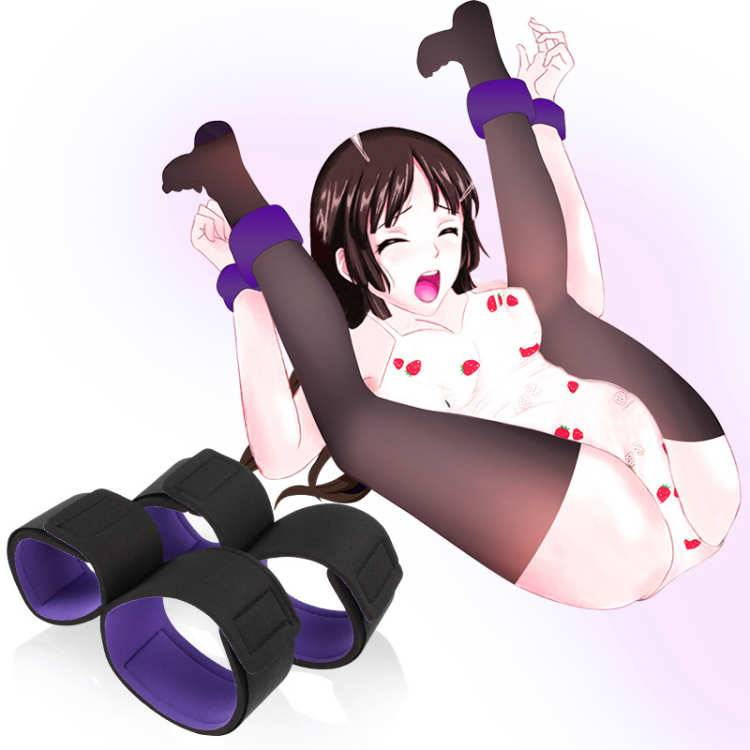
\includegraphics[width=0.42\textwidth]{images/fig_leg_spreader.jpg}\\
{\footnotesize 图：手脚捆绑器实物——绑带 + 锁扣结构，\textbf{把手腕/脚踝捆在一起}，属束缚类（bondage）。\textbf{核心风险是"血液循环 + 神经压迫"}，不是"疼不疼"。选型看\textbf{绑带软硬（选有衬垫的软带）、锁扣是否易解（带快拆/安全扣）、角度可调}（别选"死角度、松不得"的）。}
\end{center}
\par\smallskip

\noindent\textbf{使用要点（束缚类的安全底线）}：
\begin{itemize}[leftmargin=2em,itemsep=0.3em]
  \item \textbf{别勒太紧}：以"能塞进两指"为准——太紧会\textbf{压迫血管/神经}，出现\textbf{发麻、发紫、发凉、针刺感}要\textbf{立刻松}。
  \item \textbf{别压同一处过久}：同一部位束缚\textbf{不超过 20--30\,min}，\textbf{定时活动/松一松}，避免压疮/神经损伤。
  \item \textbf{避开颈/喉}：手/脚束缚\textbf{尽量在肩胛骨以下、膝盖以下}，\textbf{颈部}风险最高（压迫颈动脉/气道）。
  \item \textbf{留安全剪}：\textbf{一把快剪/安全剪随身}，意外时 10 秒内能解开；\textbf{别用"只有钥匙才能开"的锁}当入门款。
  \item \textbf{设安全词 + 保持能沟通}：束缚后\textbf{仍要能说话/摇铃/拍地}表达"停"；\textbf{别选"完全静音 + 不可动"的组合}当第一次。
  \item \textbf{皮肤检查}：有伤、湿疹、皮肤薄的人\textbf{先别束缚}该部位；\textbf{取下来看红印}（正常消退；\textbf{淤青/破皮/持续麻木}要留意）。
  \item \textbf{别在酒精/睡意下做}：痛觉和警觉都降低，\textbf{力度和时长容易失控}。
\end{itemize}

\noindent\textbf{一句话总结}：束缚/分腿器 = \textbf{限制 + 张力}；\textbf{能塞两指/避颈喉/留安全剪/每 20--30 分钟活动/取下来看红印}——记住这五点，入门就稳。

\subsection*{口球（ball gag）专项指南}

\textbf{是什么}：一个\textbf{软球（硅胶/橡胶）含在口中 + 一条系带/绳绕到脑后固定}，让含者\textbf{说不出话 + 微微有"含着东西"的紧张/失禁感 + 被束缚的顺从感}。它是 BDSM 里\textbf{偏高风险}的道具（接近 breath play）——因为球可能移位、堵住气道，\textbf{安全要求比前面几类都高}。

\begin{center}
\fbox{\parbox{0.7\textwidth}{\centering 图位预留：口球（ball gag）实物——软球 + 系带/绳绕脑后。待配图。选型看\textbf{球软不软（硅胶 > 硬塑料）、尺寸（小 > 大）、系带可否快拆、绳长留余量}。}}
\end{center}
\par\smallskip

\noindent\textbf{使用要点（高风险，安全优先）}：
\begin{itemize}[leftmargin=2em,itemsep=0.3em]
  \item \textbf{球要软、别太大}：选\textbf{硅胶软球、小尺寸}——硬球/大球\textbf{易卡喉、伤牙、堵住气道}。
  \item \textbf{必须有第二人在场}：口球\textbf{不是"独自玩"的道具}——万一球移位/含不住/误吞，\textbf{旁边必须有人能立刻取出来}。
  \item \textbf{系带/绳别太紧、留能呼吸的缝}：\textbf{能正常呼吸、能吞咽唾液}为准；\textbf{选带快拆的}（一扯就开，别用死结/钥匙锁）。
  \item \textbf{含的时间别太久}：下颌会酸、唾液增多；\textbf{每隔一会儿取出来活动一下}，别"含着一动不动半小时"。
  \item \textbf{有这些情况别用}：\textbf{吞咽困难、哮喘、气道过敏、牙/颌关节问题、醉酒/半睡}——误吞/窒息风险高。
  \item \textbf{别在完全无意识下用}：\textbf{半昏迷/深度醉酒}时含口球，\textbf{误吞风险}上升——\textbf{清醒状态下}用才安全。
  \item \textbf{取下来后别硬拽}：\textbf{沿原路慢慢取出}，检查口腔/牙齿有无压痕；\textbf{球每次用后清洗消毒}（含过唾液，多孔/软胶易藏菌）。
\end{itemize}

\noindent\textbf{一句话总结}：口球 = \textbf{说不出话 + 束缚感}；\textbf{球软且小 / 第二人在场 / 留呼吸缝 / 别含太久 / 别半昏迷下用}——这五点是安全底线，\textbf{缺了任何一条就别玩}。

\subsection*{咬夹类（乳夹 / 乳头夹 / nipple clamp）专项指南}

\textbf{是什么}：金属（不锈钢/合金）或塑料夹，两瓣咬合，夹住乳头、耳垂、脚趾、唇缘等敏感点，靠\textbf{持续压迫 + 微痛感}放大快感。日常简称"乳夹"，医学/BDSM 语境称"乳头夹"或英文 nipple clamp。常见款式：\textbf{弹簧式}（自动开合）、\textbf{旋钮式}（力度可调）、\textbf{松紧带式}（软质）。

\begin{center}
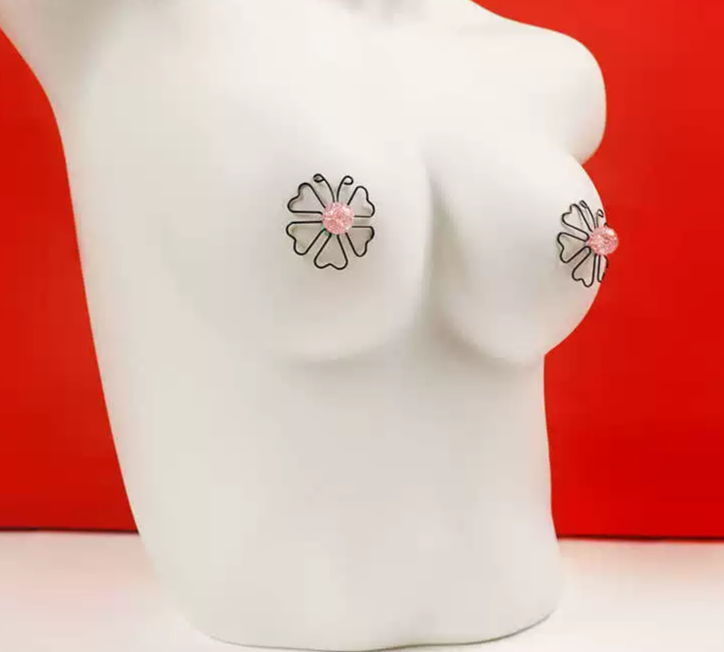
\includegraphics[width=0.32\textwidth]{images/fig_nipple_clamp.png}\\
{\footnotesize 图：乳夹（nipple clamp）实物——花瓣/蝴蝶形装饰款，两瓣咬合夹住乳头。市售乳夹\textbf{种类繁多}：功能型有弹簧式/旋钮式/松紧带式（力度可控）；\textbf{装饰型}常有蝴蝶、花瓣、爱心、皇冠、铃铛、羽毛等造型（如本图的黑色花瓣款），既夹持又兼具视觉。选型时"力度可调 + 夹口圆润不硌 + 装饰安全（无尖角）"三者兼顾，首次选\textbf{旋钮式/小号}。}
\end{center}
\par\smallskip

\begin{center}
\footnotesize
\begin{tabularx}{\textwidth}{l X X}
\toprule
\textbf{维度} & \textbf{说明} & \textbf{选择建议} \\
\midrule
材质 & 不锈钢（可加热/冷藏）/ 塑料（软、入门）& 入门选\textbf{塑料或硅胶套}（金属硬、易夹伤）；进阶选\textbf{不锈钢} \\
尺寸 & 夹口宽度 1--2\,cm & \textbf{先选小号}（夹口 1\,cm 左右），别一上来就"大号" \\
开口/松紧 & 弹簧式（自动开合）/ 旋钮式（可调）/ 松紧带式 & \textbf{旋钮式最安全}（力度可调）；弹簧式省力但\textbf{力度不易控制} \\
温度 & 可加热（40--50$^\circ$C）/ 冷藏 & 温度玩法\textbf{别太热}（先涂手背试温）；\textbf{别直接用沸水} \\
\bottomrule
\end{tabularx}
\end{center}

\noindent\textbf{使用流程（逐步）}：
\begin{enumerate}[leftmargin=2em,itemsep=0.2em]
  \item \textbf{清洁}：温水 + 中性洗涤剂清洗，\textbf{首次使用前酒精/专用消毒}（去除工业残留）。
  \item \textbf{消毒后晾干}：别用湿巾反复擦（残留刺激）。
  \item \textbf{定位}：夹在\textbf{乳头/乳晕边缘}（避开乳晕正中心，太敏感易刺痛）；也可夹\textbf{耳垂、唇缘、脚趾、手背内侧}。
  \item \textbf{力度}：\textbf{先轻夹 1--2\,min}，让对方适应；\textbf{问"还要吗？"再加重}；\textbf{别用"越紧越好"思路}。
  \item \textbf{时间}：单点\textbf{不超过 30\,min}（皮肤缺血/微血管淤血）；\textbf{多点轮换}（左右乳头交替、夹/松交替）比"死夹一个点"更舒服。
  \item \textbf{取下}：缓慢松夹、\textbf{别猛拉}（皮肤微粘/充血时猛拉易破皮）；\textbf{检查红印/淤青}（淤青 3--5 天消退属正常，\textbf{破皮/水泡/持续淤青超过 1 周}就医）。
  \item \textbf{清洁收纳}：用后清洗、晾干、\textbf{夹在软布袋/绒布套里}（金属直接放盒里会划伤/变形）。
\end{enumerate}

\noindent\textbf{安全底线}：
\begin{itemize}[leftmargin=2em,itemsep=0.2em]
  \item \textbf{避开}：破损皮肤、湿疹、皮疹、乳腺增生/结节（先咨询医生）、近期手术/穿刺点。
  \item \textbf{别用"太紧的弹簧式"入门}——力度不可调，\textbf{新手用旋钮式}或\textbf{松紧带式}更稳。
  \item \textbf{别"一边夹一边做剧烈运动"}——夹口移位会磨伤皮肤；\textbf{夹夹类玩法以"静态"为主}。
  \item \textbf{金属夹别用于"温度玩法 + 同时用力"}——金属导热快，\textbf{加热后别同时加重力度}（双重刺激易过）。
  \item \textbf{别在酒精/麻药作用下夹}——痛觉降低，\textbf{力度容易失控}（和酒精抑制勃起同理）。
  \item \textbf{孕妇/哺乳期}：乳头本身敏感，\textbf{先咨询医生}；一般建议\textbf{避开}（刺激乳头可能诱发宫缩/催乳素波动）。
\end{itemize}

\noindent\textbf{一句话总结}：乳头夹 = \textbf{持续压迫 + 微痛}的夹子类玩法；\textbf{旋钮式/小号/先轻后重/单点不超过 30 分钟/取下检查红印}——记住这五点就够用。

\section{aftercare 事后关怀（进阶的"另一半"）}
\begin{itemize}[leftmargin=2em,itemsep=0.3em]
  \item \textbf{什么是 aftercare}：高强度玩法后的\textbf{情绪 + 身体}照护——\textbf{不是"事后就散"}，是\textbf{"把峰值慢慢放下来"}。
  \item \textbf{身体}：\textbf{温水}（别冰水）、\textbf{补水}、\textbf{检查皮肤}（红印/破皮/淤青）；\textbf{别急着"起身走"}。
  \item \textbf{情绪}：\textbf{拥抱、说话、慢节奏}；\textbf{"刚才怎么样？}"比"下次再玩"更滋养；\textbf{允许"想安静一会儿"}（不用强撑"开心"）。
  \item \textbf{复盘（24--48h 后）}：\textbf{"哪个部分最让你享受？""下次想调整什么？"}——\textbf{这是把"这次"变成"下次更好"的最快方法}。
  \item \textbf{别"工具化"}：aftercare 不是"收尾任务"，是\textbf{"关系的一部分"}——\textbf{做得好，信任会累积}。
\end{itemize}

\section{一页要点}
进阶 = \textbf{更懂边界 + 更会收尾}，不是"更猛"。
\textbf{框架}：SSC（入门）$\to$PRICK（深入）——\textbf{同意可撤回、双方自愿、风险提前告知}始终成立。
\textbf{分级}：绿（感官/温度）$\to$黄（束缚/拍打）$\to$红（体压/极端温度）——\textbf{逐级升、黄级备胎、红级双人}。
\textbf{安全要点}：留剪刀/安全剪、专用体温蜡烛、别单独做体压、别"突然从背后"。
\textbf{aftercare}：温水 + 补水 + 情绪照护 + 24--48h 复盘——\textbf{"收尾"是关系的一部分}。


\end{document}
